\section{Supporting and Previous Work}
Trying to further refine orbital parameters of known systems has been done in some previous works such as Trappist-1 \cite{1704.04290}, and KOI-30 \cite{1707.04962} .
We aim to conduct a similar level of analysis for select systems, and will consider the whole ensemble of data in the long term.


A significant part of the code has already been created in this past year.
We have already coupled \reb to a few basic MCMC techniques such as 
\begin{itemize}
	\item Metropolis-Hastings (MH)
	\item Hamiltonian Monte Carlo (HMC)
	\item Affine-Invariant Sampler (emcee)
	\item Simplified Metropolis Adjusted Langevin Algorithm (SMALA)
\end{itemize}
In order to make this feat possible certain technical obstacle must be overcome.
To obtain derivatives that are stable and well behaved we require a change of coordinates.
The main reason that traditional orbital elements are not considered is due to derivative singularities in many regions of interest in the parameter space.
For example, when the eccentricity becomes zero, derivatives with respect to $\omega$ become undefined.
In order to avoid these sources of numerical instability, we use the coordinate system devised by Pal \cite{pal2009analytical}.
This coordinate system is fully analytical, and thus, is most suitible to obtain the first and second order information in a stable manner.


The SMALA method corresponds to using second order derivatives to make proposals along an N-dimensional parabola.
In order to utilize the SMALA MCMC, we also require the Hessian to be invertible.
To achieve this we introduce regularization via a general metric called softabs, which performs a softened version of an absolute value \cite{softabs}.
By applying this to the eigenvalues of the Hessian, we can assure that it is definite positive.
This modification forces SMALA's parabola proposals to have a minimum `width' which prevents proposals from going out of control when the Hessian is ill defined.
This effet is shown in figure \ref{alpha} below, where we consider a simple 1 dimensional example where we fit the mass of a 1 planet system with increasing errors.

\begin{figure}
\centering
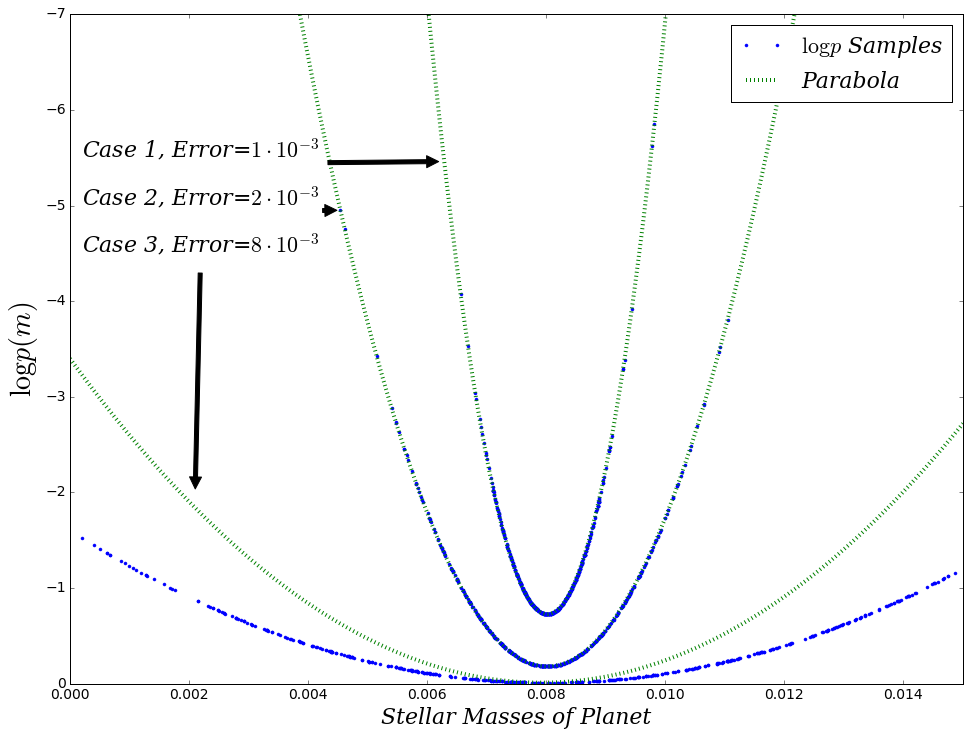
\includegraphics[width=0.75\hsize]{alpha-1.png}
   \caption{This figure shows the effect of the alpha hyper-parameter on SMALA's sampling by considering 3 cases with increasing errors. When the error is highest, in case 3, the proposed parabola is constrained due to the modified eigenvalues.
}
      \label{alpha}
\end{figure}

Increasing the error of a system geometrically corresponds to flattening the likelihood function.
A sufficently high amount of regularization, we can limit the maximum steps allowed in this less than ideal likelihood landscape.
In this limit where the derivative information is not useful, the SMALA MCMC behaves like a MH MCMC, that is, it begins to make randomly orriented proposals.
From this simple example we can see that this outcome is intuitive, the orbital parameter becomes degenerate as errors increase; the likelihood along this dimension is approaches a constant.
We are currently in the process of preparing a paper detailing our findings on the efficiency of SMALA versus the other standard MCMC considered.
In short, the brute force calculation of the Hessian via full variaitonal equations is too costly in realistic cases, however there are other possibilities to consider.
For example, we are currently working on an analytical version of SMALA which would be much faster and reduce the computational cost at least by an order of magnitude.
Another possibility is to combine various MCMC techniques and extentions of SMALA, such as empirical Hessians \cite{papamarkou2016manifold} and ensemble approaches \cite{arampatzis2016langevin} which would be similar to the emcee package. 
